\section{Code Repository}\label{codeRepository}

Code Repository

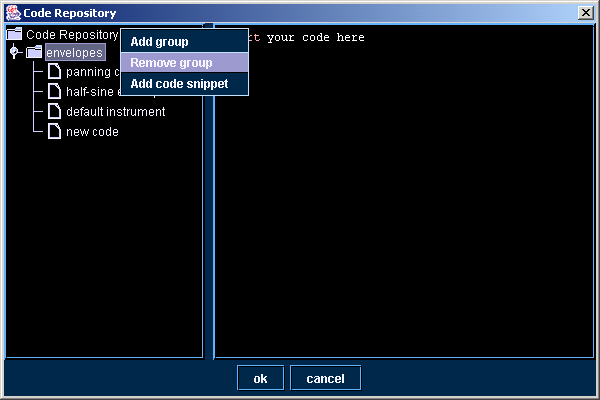
\includegraphics{images/codeRepository.png}

The Code Repository is where you edit the options that will come up from
the code popup (the popup menu that is accessible by rt-clicking on most
of the text areas in blue).

The Code Repository features a tree to organize your code. Rt-clicking
on a folder will give you options to add a new code group, remove the
current group, or add a code snippet to the group.

If you add either a code group or a code snippet it will be created with
a default name. To edit the name, double click on the group or snippet
and the area on the tree will change into a text field to edit the name.

To edit a snippet, simply click on the snippet in the tree and on the
right a text area will appear. In that text area, edit the text that is
associated with the code snippet.

When you are done editing your code repository, the next time you
rt-click on a text area, the code popup will reflect the changes you
have made, including any new code groups and snippets you've added.
